\section{Patrón de diseño: Modelo Vista Controlador}
Modelo Vista Controlador es un patrón de diseño de software el cual separa los datos de la aplicación, la interfaz de usuario y la lógica de control en tres componentes distintos.\\

\begin{itemize}
	\item \textbf{Modelo}: contiene una representación de los datos que maneja el sistema, su lógica de negocio, y sus mecanismos de persistencia.
	
	\item \textbf{Vista}: compone la información que se envía al cliente y los mecanismos interacción con éste.
	
	\item \textbf{Controlador}: actúa como intermediario entre el Modelo y la Vista, gestionando el flujo de información entre ellos y las transformaciones para adaptar los datos a las necesidades de cada uno.
\end{itemize}

La Figura \ref{fig:mvc} muestra a grandes razgos un diagrama de como opera el patrón de diseño

\begin{figure}[htbp]
	\begin{center}
		\hypertarget{fig:mvc}{
			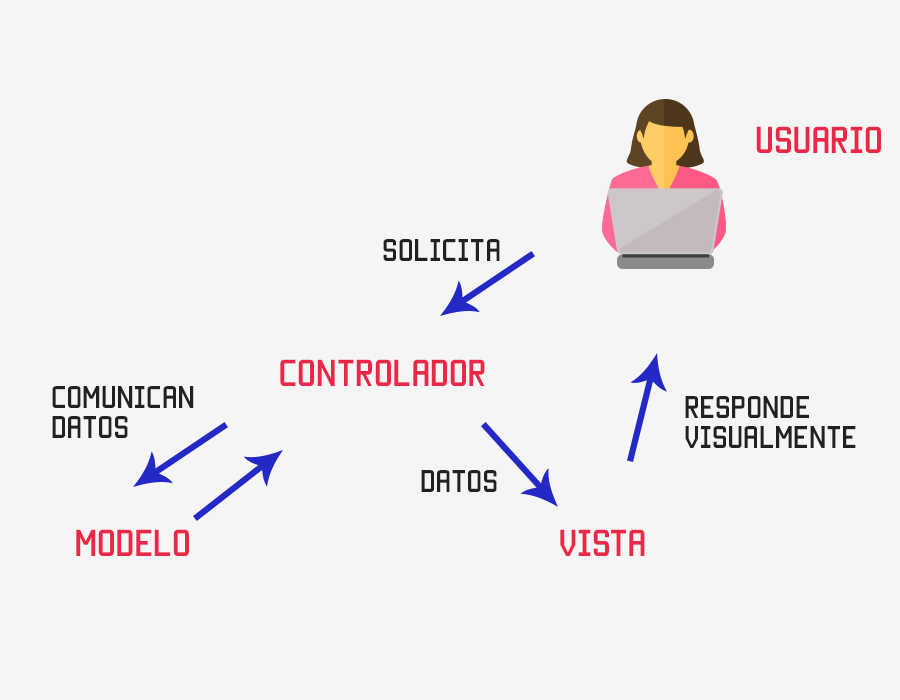
\includegraphics[scale=.3]{propuestaSolicion/turismo/images/mvc}
			\caption{Modelo Vista Controlador}
		}
		\label{fig:mvc}
	\end{center}
\end{figure}

\newpage
A continuación se describen las principales responsabilidades de cada uno de los componentes: 

\subsection{Modelo}
\begin{itemize}
	\item Se encarga de acceder a la capa de almacenamiento de datos. Idealmente el modelo debe ser independiente del sistema de almacenamiento. 
	
	\item Definir las reglas de negocio.
	
	\item Llevar un registro de las vistas y controladores del sistema.
	
	\item Notificar a las vistas los cambios que pueda producir un agente externo a los datos.
\end{itemize}

\subsection{Vista}
\begin{itemize}
	\item Recibir datos del modelo y mostrarlos al usuario.
	
	\item Tener un registro de su controlador asociado.
	
	\item Dar un servicio de actualización para que sea invocado por el controlador o por el modelo
\end{itemize}

\subsection{Controlador}
\begin{itemize}
	\item Recibir eventos de entrada.
	
	\item Contener reglas de gestón de eventos.
\end{itemize}

